\chapter{插图与绘图}\label{cha:plotting}
\section{插图}
\LaTeX{} 提供了许多定制化图片的功能。本章将会介绍如何用最常见的格式插入图片、缩放图片、旋转图片,以及如何在文档中引用这些图片。实现插入图片的功能需要在导言区引用graphics或graphicx宏包(模版已经处理好), 下面就一些重要的点展开讨论。
\begin{figure}[!hpbt]
    \centering
    \includegraphics[scale=0.25]{ntu-badgenamelogo.png}
    \caption[南通大学校名与校徽]{\enspace 南通大学校名与校徽}
    \label{fig:ntu-logo}
\end{figure}

\subsection{图片目录}
你的文档拥有很多个图片的时候,创建多个文件夹来存储图片是一个规划项目的好办法。

命令 \backslash graphicspath\{\{figures/\}\}告诉 \LaTeX{} 在 figures 文件夹中寻找图片。这个路径是当前工作文件夹的相对路径,所以编译器会在当前文档所在的目录中开始寻找文件。文件夹的路径默认情况下是相对路径,如果没有一个初始的目录被指定,例如:
\begin{verbatim}
%Path relative to the .tex file containing the \includegraphics command
\graphicspath{ {figures/} }
\end{verbatim}

这是一个非常直接的方法来指定图片所存储的路径,不过有时候会使情况变得复杂,从而导致编译器找不到图片所在的目录。所以,你最好手动指定一个对于主 ".tex" 文件来说相对的图片路径,将主 ".tex" 文件夹表示为 "./",例如:
\begin{verbatim}
%Path relative to the .tex file containing the \includegraphics command
\graphicspath{ {./figures/} }
\end{verbatim}

路径也可以是绝对路径。例如,如果你在一个本地 \LaTeX{} 环境中进行工作,你可以:
\begin{verbatim}
%Path in Windows format:
\graphicspath{ {c:/user/figures/} }
%
%Path in Unix-like (Linux, Mac OS) format
\graphicspath{ {/home/user/figures/} }
\end{verbatim}
需要注意的是,目录的结尾也需要一个斜杠,并且路径是被包含在双大括号之间。

你还可以设置多个路径,如果文档的图片被存储在多个文件夹中。例如,如果有两个文件夹figures1和figures2,使用下面的命令:
\begin{verbatim}
% There are two figure directories.
\graphicspath{ {./figures1/}{./figures2/} }
\end{verbatim}





\subsection{改变图片的大小、旋转图片}
在插入图片时,一般会涉及到额外地图片属性编辑,例如长、宽、旋转角、缩放比例等。这里给出一个使用命令 \backslash includegraphics[scale=0.1]\{ntu-badge.png\} 把图片 ntu-badge.png 插入到文档中的简单例子,额外的参数scale=0.1会把图片的大小变为原本的0.1倍:
\begin{figure}[!hpbt]
\begin{minipage}{0.5\textwidth}
\begin{lstlisting}[language=tex]
\includegraphics[scale=0.1]{ntu-badge.png}
\end{lstlisting}%
\end{minipage}
\begin{minipage}{0.45\textwidth}
\centering
\includegraphics[scale=0.1]{ntu-badge.png}
\end{minipage}
\end{figure}

你也可以指定图片的宽度和高度,其方法为通过方括号里的参数[width=4cm, height=4cm]定义,可以使用不同的单位。如果只有宽度 width 被指定了,那么高度会被自动地按照图片原始比例设置。
\begin{figure}[!hpbt]
\begin{minipage}{0.5\textwidth}
\begin{lstlisting}[language=tex]
\includegraphics[width=4cm, height=4cm]{ntu-badge.png}
\end{lstlisting}%
\end{minipage}
\begin{minipage}{0.45\textwidth}
\centering
\includegraphics[width=4cm, height=4cm]{ntu-badge.png}
\end{minipage}
\end{figure}

长度单位也可以被设置为文档中某些属性的相对值。例如,你可以将图片的宽度设置为文档中一行文本所占的宽度:
\begin{figure}[!hpbt]
\begin{minipage}{0.5\textwidth}
\begin{lstlisting}[language=tex]
\includegraphics[width=\textwidth]{ntu-badge.png}
\end{lstlisting}%
\end{minipage}
\begin{minipage}{0.45\textwidth}
\centering
\includegraphics[width=\textwidth]{ntu-badge.png}
\end{minipage}
\end{figure}

除了 \backslash textwidth ,你还可以使用其他的 \LaTeX{} 默认长度,例如 \backslash columnsep 、 \backslash linewidth 、 \backslash textheight 、 \backslash paperheight 等。

LaTeX 中还有一种常见的改变图片的方法,下面对图片执行0.1倍缩放和逆时针旋转$45^{\circ}$,顺时针旋转的话你可以使用负数:
\begin{figure}[!hpbt]
\begin{minipage}{0.5\textwidth}
\begin{lstlisting}[language=tex]
\includegraphics[scale=0.1, angle=45]{ntu-badge.png}
\end{lstlisting}%
\end{minipage}
\begin{minipage}{0.45\textwidth}
\centering
\includegraphics[scale=0.1, angle=45]{ntu-badge.png}
\end{minipage}
\end{figure}

\subsection{插入位置}
我们介绍了如何在文档中插入图片,但是文字和图片的结合可能并不是我们想要的样子。所以我们接下来介绍一种新的figure环境。
\begin{verbatim}
\begin{figure}[h]
\includegraphics[width=8cm]{ntu-badge.png}
\end{figure}
\end{verbatim}
figure环境的作用是在文档中将图片展示为浮动元素。这意味着你可以把图片放置在figure环境之中,不需要再去关注图片的位置,\LaTeX{} 会自动把图片放置在文档中的合适位置。

当然,有些时候我们需要更细致地控制图片的位置。figure环境中额外的位置控制参数为我们提供了一套控制图片位置的方法。下面我们给出一个简单的例子。
\begin{table}[!hpbt]
    \caption[图片插入位置控制选项]{\enspace 图片插入位置控制选项}
    \label{tab:figure-position-options}
    \centering
    \normalsize% fontsize 
    \setlength{\tabcolsep}{4pt}% column separation
    \begin{tabular}{ll}
    \toprule
    选项 & 位置 \\
    \midrule
    h	& 将浮动元素的位置设定为 here\\
    t	& 将浮动元素的位置设定为页面的上方(top)\\
    b	& 将浮动元素的位置设定为页面的底部(bottom)\\
    p	& 将浮动元素仅放置在一个特殊的页面\\
    !	& 重新设置 \LaTeX{} 的一个内部参数\\
    H	& 浮动元素精确地放置在文本中所出现的位置\\
    \bottomrule
    \end{tabular}
\end{table}
其中, \backslash begin\{figure\}[h],方括号中的参数h意味着 here,即大约插入到当前上下文位置,而不是完全精确地插入到给定位置。 参数 ! 决定了 \LaTeX{} 如何判断一个浮动元素的位置够不够“好”,参数 H 需要引入float包,它有可能会造成一些错误,有时候等价于h!。表~\ref{tab:figure-position-options}~中列出了参数的可选值。

\subsection{图题、标签、引用}
让我们回顾本节第一个图片例子(图\ref{fig:ntu-logo}),其代码如下:
\begin{verbatim}
\begin{figure}[!hpbt]
    \centering
    \includegraphics[scale=0.25]{ntu-badgenamelogo.png}
    \caption[南通大学校名与校徽]{\enspace 南通大学校名与校徽}
    \label{fig:ntu-logo}
\end{figure}
\end{verbatim}
这里需要注意几个命令:(1)命令 \backslash centering 会将图片居中显示,默认的对齐选项是向左对齐;(2)命令 \backslash caption\{Some caption\} 就是制作图题的命令,在大括号内输入你要添加的图题文字就可以了,命令的位置决定着图题会出现在图片的上方或者下方,这里出现在下方;(3)命令 \backslash label\{\} 是给图片打标签,用于内部图片索引,大括号内需要填入唯一索引字符串,如“fig:ntu-logo”,对图片标签添加一个前缀“fig:”是一个很好的习惯;(4)要引用这个图片,命令很简单:  \backslash ref\{fig:ntu-logo\} ,即如图
\ref{fig:ntu-logo};(5)可以使用命令 \backslash pageref\{fig:ntu-logo\} 获取图片所在页码,即图\ref{fig:ntu-logo}在本文第\pageref{fig:ntu-logo}页。如果你想要引用一个图片,那么 \backslash caption命令是强制的,并且 \backslash label 命令位于 \backslash caption 之后。

\LaTeX{} 另外一个强大的功能是,你可以自动生成文档中图片的列表:
\begin{verbatim}
\listoffigures
\end{verbatim}
这个命令仅对有标签的图片有效。重要提示:你必须编译 \LaTeX{} 文档两次来使交叉引用等功能正常显示。

\subsection{不同分辨率图片}
我们在 \backslash includegraphics 命令中输入图片的文件名的时候,会忽略了片文件的扩展名。事实上,添加扩展名并不是强制的,尽管很多时候添加扩展名是很有用的。如果没有给出文件扩展名,那么 \LaTeX{} 会在当前文件夹中自动搜索所有支持的文件格式,并且会用默认的顺序来搜索各种扩展名(这个顺序可以自定义)。

如果你需要经常在开发模式和生产模式之间切换,那么这个功能会很有用。在开发模式中(当文档还没有完成的时候),你可能想去使用低分辨率的图片(一般来说是png格式的)来加速编译。在生产模式中(生成文档的最终版本),你可能想要使用高分辨率的图片。

你可以这样做:(1)不要在 \backslash includegraphics 命令中输入文件的扩展名,(2)在文档的导言区设定你想要的扩展名。这样,我们可以在图片的两种格式之间灵活切换,例如 venndiagram.pdf(高分辨率)和 venndiagram.png(低分辨率)。然后我们可以在导言区使用下面的命令:
\begin{verbatim}
\DeclareGraphicsExtensions{.png,.pdf}
\end{verbatim}
上面的命令的作用是:如果在同一位置中,两个具有相同文件名而扩展名不同的文件(例如venndiagram.pdf和venndiagram.png)同时存在,那么扩展名位置在前的文件将会被优先使用(这个例子中的png);如果没有png文件,那么pdf文件会被使用。

当文档完成之后,为了使用高分辨率的pdf图片,我们可以更换后缀的顺序:
\begin{verbatim}
\DeclareGraphicsExtensions{.pdf,.png}
\end{verbatim}
如果pdf图片还没有转换为png格式,我们可以在 \LaTeX{} 中直接生成低分辨率的png图片。我们首先在导言区 \backslash usepackage\{graphicx\}(本模版不需要用户额外再引入宏包)命令之后添加下面的命令:
\begin{verbatim}
\usepackage{epstopdf}
\epstopdfDeclareGraphicsRule{.pdf}{png}{.png}{convert #1 \OutputFile}
\DeclareGraphicsExtensions{.png,.pdf}
\end{verbatim}
如果venndiagram2.pdf存在,但是venndiagram2.png不存在,那么编译器会自动生成低分辨率的图像文件venndiagram2-pdf-converted-to.png。命令 \texttt{convert \#1} 用来执行转换操作,你也可以对它添加额外的参数,例如 \texttt{convert \-density 100 \#1} 。

这里需要注意:我们在执行pdflatex 命令的时候,需要添加 \texttt{--shell-escape} 参数,以确保能够自动转换出低分辨率的图片。
对于最终的正式版,我们必须把 \backslash epstopdfDeclareGraphicsRule 命令注释掉,以确保高分辨率的图片会被加载。同时,我们还需要改变加载扩展名优先级的顺序。


\section{绘图}
为帮助您快速上手 TikZ,本说明省去了冗长的安装与配置,同时避免过度深入技术细节。此部分主要包含使用 TikZ 绘制图形时的操作指导建议与样例。更详细的内容可参见 \href{https://tikz.dev/tutorials-guidelines}{PGF/TikZ Manual}。

本教程面向TikZ新用户,内容并非涵盖所有功能特性,仅聚焦于您可能立即用到的核心功能。

卡尔是位高中数学兼化学教师,过去常使用 \LaTeX{} 的picture环境为讲义和试卷绘制图形。虽然效果尚可,但绘图过程往往耗时冗长,且常出现线条角度微偏、圆形难以精准绘制等问题。当然,学生们对线条角度是否精确毫不在意——无论图形绘制得多精美,他们总认为卡尔的试题太难。但卡尔自己从未对绘制效果完全满意。

卡尔的儿子(他对效果更不满意,毕竟他不用参加考试)建议父亲尝试新绘图宏包。令人困惑的是,这个宏包似乎有两个名字:卡尔先下载安装了名为pgf的宏包,随后发现其中还包含另一个叫TikZ的宏包——其名称源自"TikZ ist kein Zeichenprogramm"(TikZ非绘图工具)的递归缩写。卡尔觉得这有些古怪,TikZ的名字似乎暗示该工具无法满足他的需求。不过长期使用GNU软件的经验让他想到"GNU也不是Unix的缩写"(GNU's Not Unix),事情或许还有转机。儿子向他保证:TikZ的名称旨在提醒用户,这不是能用鼠标或数位板直接绘图的软件,而更像一种"图形语言"。

\begin{example}卡尔计划在下一份讲义中为学生添加图示。他当前正在讲授正弦与余弦函数,期望绘制的图形能达到图\ref{fig:karl-sine-problem}的理想效果:
\begin{figure}[!hpbt]
    \centering
    \includegraphics[scale=0.75]{doc/figures/image-5.png}
    \caption[卡尔设想的三角函数效果图]{\enspace 卡尔设想的三角函数效果图}
    \label{fig:karl-sine-problem}
\end{figure}
\end{example}


本模版已经集成TikZ宏包,在引入样式宏包cnbasesetup.sty时,传入\texttt{tikz}参数引入TikZ绘图宏包。
\begin{verbatim}
    \usepackage[super,tikz,tab,list,math]{style/cnbasesetup}
\end{verbatim}
在TikZ中绘制图形时,需在起始处告知 \TeX 或 \LaTeX{} 系统准备开始绘图。
\LaTeX{} 环境下需使用\{tikzpicture\}环境,而原生 \TeX{} 中则通过\backslash tikzpicture 命令启动绘图,并以 \backslash endtikzpicture 命令结束。

Karl 使用 \LaTeX{} 绘制了一个简单图形以测试环境。
\begin{figure}[!hpbt]
\begin{minipage}{0.5\textwidth}
\begin{lstlisting}[language=tex]
\begin{tikzpicture}
    \draw (-1.5,0)-- (1.5,0);
    \draw (0,-1.5)-- (0,1.5);
\end{tikzpicture}
\end{lstlisting}%
\end{minipage}
\begin{minipage}{0.45\textwidth}
\centering
 \begin{tikzpicture}
     \draw (-1.5,0)-- (1.5,0);
     \draw (0,-1.5)-- (0,1.5);
 \end{tikzpicture}
\end{minipage}
\end{figure}

诚然,当前尚未完成完整图形,但坐标系已然建立。准确地说,我们已绘制出构成坐标轴的基准线。卡尔突然产生不祥预感——距离目标效果尚有差距。

深入解析这段代码:首先加载了TikZ宏包,该宏包是基础pgf系统的"前端"封装层。本手册不会介绍更为底层的基础层功能,其使用难度也更高,TikZ前端层通过提供简洁语法显著降低了操作门槛。

在\{tikzpicture\}环境中存在两条 \backslash draw 指令,其含义是:"该命令后方至分号间定义的路径应被绘制出来"。第一条路径定义为(-1.5,0) -- (1.5,0),即"从坐标位置(-1.5,0)到(1.5,0)的直线段"。此处坐标采用特殊坐标系表示,初始状态下1单位长度对应1厘米。

卡尔欣慰地注意到,该绘图环境能智能地预留充足空间容纳整个图形。

下面给出几种常用的绘图基础操作。
\begin{enumerate}
    \item \emph{直线路径创建} ~~在TikZ中,path(路径)是所有图形的基本构成单元。所谓路径,即由相互连接的直线段与曲线构成的序列(虽非完整定义,但暂可忽略复杂变体)。创建路径时需以圆括号包裹起始坐标点,如(0,0)。其后可添加一系列"path(路径)延展操作符",其中最简单的延展符——即我们已使用的"--"符号——必须后接新坐标点,表示将路径沿直线延伸至该位置。例如,若将两条坐标轴路径合并为一条,其代码实现如下:
    \begin{figure}[!hpbt]
    \begin{minipage}{0.5\textwidth}
    \begin{lstlisting}[language=tex]
    \tikz \draw (-1.5,0) -- (1.5,0) -- (0,-1.5) -- (0,1.5);
    \end{lstlisting}%
    \end{minipage}
    \begin{minipage}{0.45\textwidth}
    \centering
    \tikz \draw (-1.5,0) -- (1.5,0) -- (0,-1.5) -- (0,1.5);
    \end{minipage}
    \end{figure}

    卡尔对当前未使用 \{tikzpicture\} 环境稍感困惑——此处改用精简命令 \backslash tikz实现。该命令存在两种调用形式:其一接收单参数(以左花括号起始,如 \backslash tikz\{ \backslash draw (0,0) -- (1.5,0)\},输出效果为 \tikz{\draw (0,0) -- (1.5,0)} );其二则自动收集分号前的所有内容并置入 \{tikzpicture\} 环境。经验法则表明:所有TikZ绘图命令必须作为 \backslash tikz 命令的参数,或置于 \{tikzpicture\} 环境内部。所幸 \backslash draw 命令仅在该环境内有效定义,几乎可避免意外出错。
    
    \item \emph{曲线路径创建} ~~接下来卡尔要绘制圆形,直线段显然行不通。为此TikZ提供了专用曲线语法,需要借助一至两个"控制点"。其数学背景并非完全平凡,但核心原理可简述如下:假设起点为$x$,第一控制点为$y$,则曲线在$x$点处的切线方向指向$y$;若终点为$z$且第二支撑点为$w$,则曲线将终止于$z$点,并在该点形成指向$w$的切线方向。

    在TikZ中实现曲线路径延展的通用语法为:\texttt{.. controls ⟨第一控制点⟩ and ⟨第二控制点⟩ .. ⟨终点⟩ }。若省略and ⟨第二控制点⟩参数,系统将自动复用第一控制点。示例如下(为清晰起见额外标注了控制点):
    \begin{figure}[!hpbt]
    \begin{minipage}{0.5\textwidth}
    \centering
    \begin{lstlisting}[language=tex]
    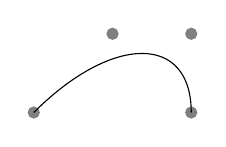
\begin{tikzpicture}
    \filldraw [gray] (0,0) circle [radius=2pt]
            (1,1) circle [radius=2pt]
            (2,1) circle [radius=2pt]
            (2,0) circle [radius=2pt];
    \draw (0,0) .. controls (1,1) and (2,1) .. (2,0);
    \end{tikzpicture}
    \end{lstlisting}%
    \end{minipage}
    \begin{minipage}{0.45\textwidth}
    \centering
    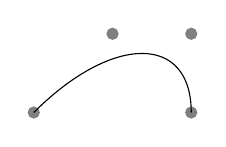
\begin{tikzpicture}
            \filldraw [gray] (0,0) circle [radius=2pt]
                   (1,1) circle [radius=2pt]
                   (2,1) circle [radius=2pt]
                   (2,0) circle [radius=2pt];
            \draw (0,0) .. controls (1,1) and (2,1) .. (2,0);
        \end{tikzpicture}
    \end{minipage}
    \end{figure}

    因此卡尔采用这曲线绘制种方式,仅仅通过精确调整曲线绘制参数实现了半圆的绘制。卡尔对结果颇感满意,但发现以这种方式指定圆形绘制极其繁琐。
    \begin{figure}[!hpbt]
    \begin{minipage}{0.5\textwidth}
    \centering
    \begin{lstlisting}[language=tex]
    \begin{tikzpicture}
        \draw (-1.5,0) -- (1.5,0);
        \draw (0,-1.5) -- (0,1.5);
        \draw (-1,0) .. controls (-1,0.555) and (-0.555,1) .. (0,1)
               .. controls (0.555,1) and (1,0.555) .. (1,0);
    \end{tikzpicture}
    \end{lstlisting}%
    \end{minipage}
    \begin{minipage}{0.45\textwidth}
    \centering
    \begin{tikzpicture}
        \draw (-1.5,0) -- (1.5,0);
        \draw (0,-1.5) -- (0,1.5);
        \draw (-1,0) .. controls (-1,0.555) and (-0.555,1) .. (0,1)
               .. controls (0.555,1) and (1,0.555) .. (1,0);
    \end{tikzpicture}
    \end{minipage}
    \end{figure}

    

    \item \emph{圆路径创建} ~~幸运的是,存在更为简洁的实现方式。我们可使用路径构建操作符\texttt{circle}简洁高效准确地绘制圆形。操作符\texttt{circle}后接方括号以包裹半径值(如下例所示)。需注意:该操作会将当前路径点作为圆心。
    \begin{figure}[!hpbt]
    \begin{minipage}{0.5\textwidth}
    \begin{lstlisting}[language=tex]
    \tikz \draw (0,0) circle [radius=10pt];
    \end{lstlisting}%
    \end{minipage}
    \begin{minipage}{0.45\textwidth}
    \centering
    \tikz \draw (0,0) circle [radius=10pt];
    \end{minipage}
    \end{figure}

    此外,您还可通过ellipse操作符向路径追加椭圆。该操作需指定两个半径值(而非单个半径),语法如下:
    \begin{figure}[!hpbt]
    \begin{minipage}{0.5\textwidth}
    \begin{lstlisting}[language=tex]
    \tikz \draw (0,0) ellipse [x radius=20pt, y radius=10pt];
    \end{lstlisting}%
    \end{minipage}
    \begin{minipage}{0.45\textwidth}
    \centering
    \tikz \draw (0,0) ellipse [x radius=20pt, y radius=10pt];
    \end{minipage}
    \end{figure}

    要绘制轴线非水平或垂直方向的椭圆(即类似右图的"旋转椭圆"),您可运用旋转变换实现(变换机制将在后续章节详解)。这里我们给出绘制代码示例,如下:\begin{verbatim}\tikz \draw[rotate=30] (0,0) ellipse [x radius=6pt, y radius=3pt];\end{verbatim}

    因此,回到卡尔的绘图需求,他只需书写 \texttt{ \backslash draw (0,0) circle [radius=1cm];} 即可完成圆形绘制。然而,卡尔此时警觉地发现:当前圆形尺寸过小,而最终图形需大幅放大。所幸TikZ具备强大的变换选项功能,只需按三倍比例缩放即可轻松实现。但为节省此处版面,我们暂保持当前尺寸不变。
    \begin{figure}[!hpbt]
    \begin{minipage}{0.5\textwidth}
    \begin{lstlisting}[language=tex]
    \begin{tikzpicture}
    \draw (-1.5,0) -- (1.5,0);
    \draw (0,-1.5) -- (0,1.5);
    \draw (0,0) circle [radius=1cm];
    \end{tikzpicture}
    \end{lstlisting}%
    \end{minipage}
    \begin{minipage}{0.45\textwidth}
    \centering
    \begin{tikzpicture}
    \draw (-1.5,0) -- (1.5,0);
    \draw (0,-1.5) -- (0,1.5);
    \draw (0,0) circle [radius=1cm];
    \end{tikzpicture}
    \end{minipage}
    \end{figure}

    
    \item \emph{长方形路径创建} ~~接下来我们需要添加背景网格。存在多种实现方案,例如绘制大量矩形。鉴于矩形应用广泛,TikZ提供了专用语法:向当前路径追加矩形时,请使用\texttt{rectangle}路径构建操作符。该操作符需后接另一坐标点,系统将自动把前一坐标点与当前坐标点作为矩形对角顶点,构建矩形路径。因此,让我们在图形中添加两个矩形示例:
    \begin{figure}[!hpbt]
    \begin{minipage}{0.5\textwidth}
    \begin{lstlisting}[language=tex]
    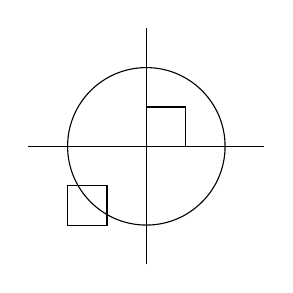
\begin{tikzpicture}
    \draw (-1.5,0) -- (1.5,0);
    \draw (0,-1.5) -- (0,1.5);
    \draw (0,0) circle [radius=1cm];
    \draw (0,0) rectangle (0.5,0.5);
    \draw (-0.5,-0.5) rectangle (-1,-1);
    \end{tikzpicture}
    \end{lstlisting}%
    \end{minipage}
    \begin{minipage}{0.45\textwidth}
    \centering
    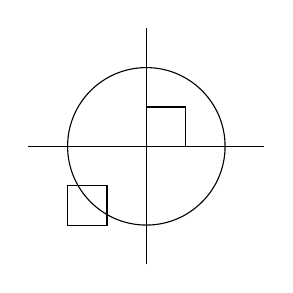
\begin{tikzpicture}
    \draw (-1.5,0) -- (1.5,0);
    \draw (0,-1.5) -- (0,1.5);
    \draw (0,0) circle [radius=1cm];
    \draw (0,0) rectangle (0.5,0.5);
    \draw (-0.5,-0.5) rectangle (-1,-1);
    \end{tikzpicture}
    \end{minipage}
    \end{figure}

    尽管通过矩形命令绘制网格是一个理论可行的方法,但是对于类似卡尔这种绘制较多矩形构成网格的问题不是一个好的解决方案,并且这种方法无法实现"未闭合"的边界。因此卡尔的问题遇到了一点困难。正当卡尔欲采用另一种笨办法——使用 \backslash draw 命令直接绘制四条横竖直线时,却意外发现存在专用的grid路径构建操作符。

    \item \emph{网格形路径创建} ~~grid路径操作符可在当前路径中添加网格。该操作会以前一坐标点为起点,后接坐标点为终点形成一个矩形区域,并自动为该矩形区域生成填充的网格线。例如,代码
    \begin{verbatim}
        \tikz \draw[step=2pt] (0,0) grid (10pt,10pt);
    \end{verbatim} 
    将生成如右图所示的网格(请注意通过 \backslash draw 的可选参数step可定义网格间距,另有xstep与ystep参数可分别设置横纵间距)。卡尔很快会发现,这类参数能实现丰富的样式控制。

    针对卡尔的需求,可采用以下代码实现:
    \begin{figure}[!hpbt]
    \begin{minipage}{0.5\textwidth}
    \begin{lstlisting}[language=tex]
    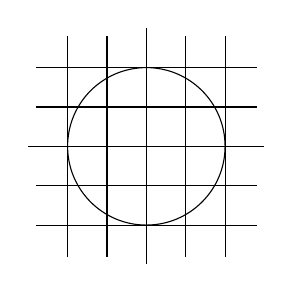
\begin{tikzpicture}
    \draw (-1.5,0) -- (1.5,0);
    \draw (0,-1.5) -- (0,1.5);
    \draw (0,0) circle [radius=1cm];
    \draw[step=.5cm] (-1.4,-1.4) grid (1.4,1.4);
    \end{tikzpicture}
    \end{lstlisting}%
    \end{minipage}
    \begin{minipage}{0.45\textwidth}
    \centering
    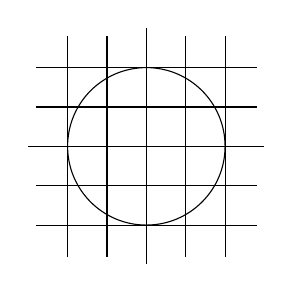
\begin{tikzpicture}
    \draw (-1.5,0) -- (1.5,0);
    \draw (0,-1.5) -- (0,1.5);
    \draw (0,0) circle [radius=1cm];
    \draw[step=.5cm] (-1.4,-1.4) grid (1.4,1.4);
    \end{tikzpicture}
    \end{minipage}
    \end{figure}

    再次审视目标图形时,卡尔意识到网格线应当更加淡化(其子曾提醒:未经淡化的网格线容易分散注意力)。为此,他在绘制网格的\backslash draw命令中追加两个参数:首先将线条颜色设为灰色,其次将线宽调整为极细。最终调整命令顺序,优先绘制网格使其成为底层元素。
    \begin{figure}[!hpbt]
    \begin{minipage}{0.5\textwidth}
    \begin{lstlisting}[language=tex]
    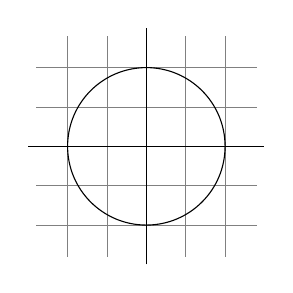
\begin{tikzpicture}
    \draw[step=.5cm,gray,very thin] (-1.4,-1.4) grid (1.4,1.4);
    \draw (-1.5,0) -- (1.5,0);
    \draw (0,-1.5) -- (0,1.5);
    \draw (0,0) circle [radius=1cm];
    \end{tikzpicture}
    \end{lstlisting}%
    \end{minipage}
    \begin{minipage}{0.45\textwidth}
    \centering
    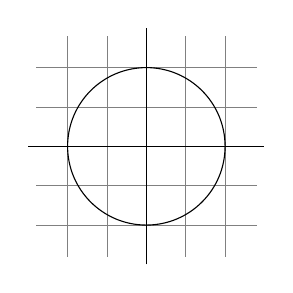
\begin{tikzpicture}
    \draw[step=.5cm,gray,very thin] (-1.4,-1.4) grid (1.4,1.4);
    \draw (-1.5,0) -- (1.5,0);
    \draw (0,-1.5) -- (0,1.5);
    \draw (0,0) circle [radius=1cm];
    \end{tikzpicture}
    \end{minipage}
    \end{figure}

    \item \emph{样式化应用技巧} ~~卡尔可采用预定义样式help lines 替代直接使用gray,very thin参数。样式是预置的绘图参数集合,能系统化管理图形外观。调用help lines即表示"使用预设的辅助线绘制样式"。若卡尔后续想将网格线改为半透明蓝色(blue!50),只需在任意位置添加如下样式定义:
    \begin{verbatim} help lines/.style={color=blue!50,very thin} \end{verbatim}
    该"样式设定器"的效果是:在当前作用域或环境中,help lines选项将完全等同于color=blue!50,very thin的参数组合。

    使用样式能显著提升图形代码的灵活性,让您以统一的方式轻松调整外观效果。通常建议在\{tikzpicture\}环境起始处定义样式,但若需全文档统一风格,可在文档导言区使用 \backslash tikzset命令进行全局样式定义:
    \begin{verbatim} \tikzset{help lines/.style=very thin} \end{verbatim}

    要构建层级化的样式体系,您可以让一个样式继承另一个样式的特性。例如,若卡尔需要基于标准网格样式创建专属的"Karl's grid"样式,可通过以下方式定义
    \begin{verbatim} 
        \tikzset{Karl's grid/.style={help lines,color=blue!50}}
        ...
        \draw[Karl's grid] (0,0) grid (5,5);
    \end{verbatim}

    通过参数化机制,样式的功能变得更加强大。这意味着样式可以像其他选项一样接收参数。例如,卡尔可以将其网格样式参数化——默认显示为蓝色,同时保留切换其他颜色的灵活性:
    \begin{verbatim} 
    \begin{tikzpicture}
    [Karl's grid/.style ={help lines,color=#1!50},
    Karl's grid/.default=blue]

    \draw[Karl's grid]     (0,0) grid (1.5,2);
    \draw[Karl's grid=red] (2,0) grid (3.5,2);
    \end{tikzpicture}
    \end{verbatim}

    在此示例中,`Karl's grid`样式被定义为 \{tikzpicture\}环境的可选参数。如需为其他元素添加样式,只需以逗号分隔继续追加。当存在多个样式定义时,环境的可选参数长度很可能超过实际的绘图内容本身。

    \item \emph{绘图选项} ~~
    卡尔希望了解影响路径绘制的其他选项。他已发现color=⟨颜色⟩可设置线条颜色,而draw=⟨颜色⟩功能类似但更专注——它仅控制线条颜色,填充色可单独设定(这在后续绘制角度弧线填充时将用到)。

    他注意到very thin样式生成极细线条。对此卡尔毫不意外,正如他平静接受以下事实:thin生成细线,thick生成粗线,very thick生成加粗线,ultra thick生成超粗线,而ultra thin生成的线条则细到低分辨率打印设备和显示器难以呈现。此刻他思考:究竟何种选项能产生"标准"粗细的线条?事实证明thin正是正确选择——其粗细与 \TeX 的 \backslash hrule命令完全一致。不过卡尔仍想探究是否存在介于细线与粗线之间的"中间值"。答案是肯定的:semithick。

    另一种实用的线条处理方式是虚线或点线绘制。通过dashed(虚线)与dotted(点线)样式即可实现(效果分别见右图A、B)。这两种样式均提供疏松与致密变体:loosely dashed(疏松虚线)、densely dashed(致密虚线)、loosely dotted(疏松点线)及densely dotted(致密点线)。若确有特殊需求,卡尔还可通过dash pattern选项自定义复杂虚线模式——但其子坚决主张虚线应极度谨慎使用,因过度使用易分散注意力。他断言复杂虚线模式实属糟糕,而卡尔的学生们则对虚线样式毫不在意。

    \vskip \baselineskip
    \item \emph{弧形路径创建} ~~
    当前的技术难点是绘制角度弧线。arc路径构建操作符可解决此需求——它能绘制圆形或椭圆的部分弧段。该操作符后需接方括号包裹的弧线参数,例如arc[start angle=10, end angle=80, radius=10pt]的含义不言自明。卡尔明确需要绘制从 $\alpha$ 到 $\beta$ 的弧线(如右图),其半径应相对较小(约为圆半径的三分之一)。需特别注意:使用arc操作符时,系统将以当前位置为弧线起点进行绘制,因此我们需先定位至起点坐标。
    \begin{figure}[!hpbt]
    \begin{minipage}{0.5\textwidth}
    \begin{lstlisting}[language=tex]
    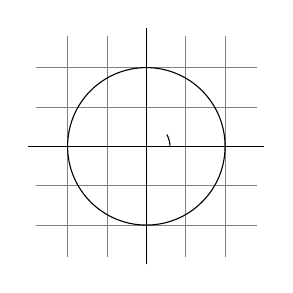
\begin{tikzpicture}
    \draw[step=.5cm,gray,very thin] (-1.4,-1.4) grid (1.4,1.4);
    \draw (-1.5,0) -- (1.5,0);
    \draw (0,-1.5) -- (0,1.5);
    \draw (0,0) circle [radius=1cm];
    \draw (3mm,0mm) arc [start angle=0, end angle=30, radius=3mm];
    \end{tikzpicture}
    \end{lstlisting}%
    \end{minipage}
    \begin{minipage}{0.45\textwidth}
    \centering
    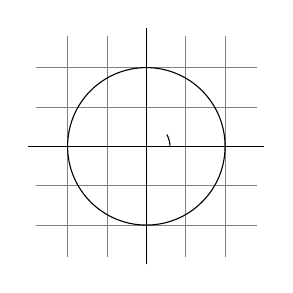
\begin{tikzpicture}
    \draw[step=.5cm,gray,very thin] (-1.4,-1.4) grid (1.4,1.4);
    \draw (-1.5,0) -- (1.5,0);
    \draw (0,-1.5) -- (0,1.5);
    \draw (0,0) circle [radius=1cm];
    \draw (3mm,0mm) arc [start angle=0, end angle=30, radius=3mm];
    \end{tikzpicture}
    \end{minipage}
    \end{figure}

    卡尔认为当前图形确实略显局促,若未掌握缩放技巧将难以继续操作。为此,他可为环境添加[scale=2]缩放选项。虽然可单独应用于每条 \backslash draw命令,但此方案略显繁琐。取而代之的是,将其添加至整个 \{ tikzpicture \} 环境,即可使缩放效果作用于环境内所有元素:
    \begin{figure}[!hpbt]
    \begin{minipage}{0.5\textwidth}
    \begin{lstlisting}[language=tex]
    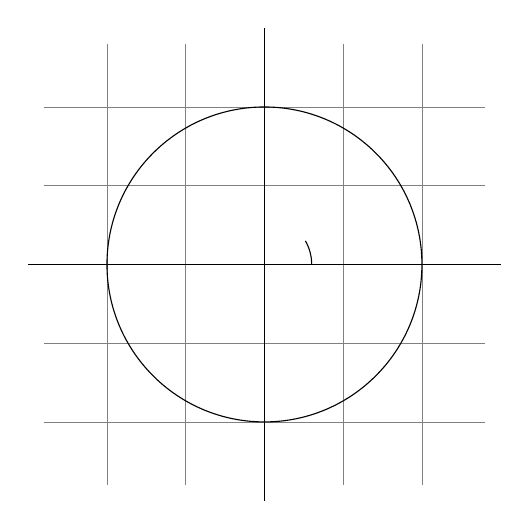
\begin{tikzpicture}[scale=2]
    \draw[step=.5cm,gray,very thin] (-1.4,-1.4) grid (1.4,1.4);
    \draw (-1.5,0) -- (1.5,0);
    \draw (0,-1.5) -- (0,1.5);
    \draw (0,0) circle [radius=1cm];
    \draw (3mm,0mm) arc [start angle=0, end angle=30, radius=3mm];
    \end{tikzpicture}
    \end{lstlisting}%
    \end{minipage}
    \begin{minipage}{0.45\textwidth}
    \centering
    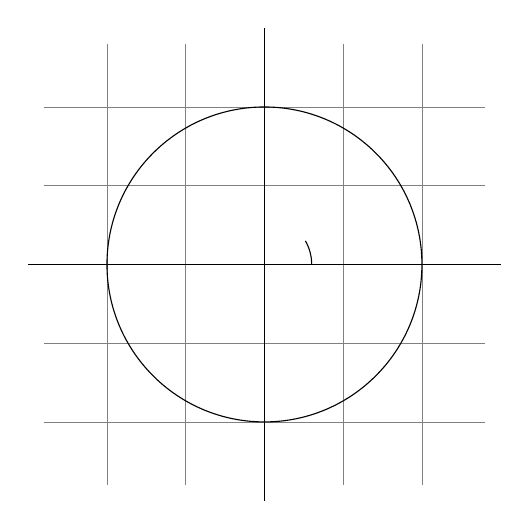
\begin{tikzpicture}[scale=2]
    \draw[step=.5cm,gray,very thin] (-1.4,-1.4) grid (1.4,1.4);
    \draw (-1.5,0) -- (1.5,0);
    \draw (0,-1.5) -- (0,1.5);
    \draw (0,0) circle [radius=1cm];
    \draw (3mm,0mm) arc [start angle=0, end angle=30, radius=3mm];
    \end{tikzpicture}
    \end{minipage}
    \end{figure}

    对于椭圆弧的绘制,您可通过指定"两个"半径参数来实现(区别于标准圆弧的单一半径参数)。例如:
    \begin{figure}[!hpbt]
    \begin{minipage}{0.5\textwidth}
    \begin{lstlisting}[language=tex]
    \tikz \draw (0,0)
    arc [start angle=0, end angle=315,
         x radius=1.75cm, y radius=1cm];
    \end{lstlisting}%
    \end{minipage}
    \begin{minipage}{0.45\textwidth}
    \centering
    \tikz \draw (0,0)
    arc [start angle=0, end angle=315,
         x radius=1.75cm, y radius=1cm];
    \end{minipage}
    \end{figure}
    \item \emph{路径裁剪} ~~
    为精简本手册版面,建议对卡尔的图形进行局部裁剪,从而聚焦呈现"关键"区域。在TikZ中实现裁剪相当便捷:只需使用 \backslash clip命令即可裁剪后续所有绘图内容。该命令语法与 \backslash draw类似,但不会实际绘制路径,而是将给定路径设为裁剪边界作用于后续图形元素。
    \begin{figure}[!hpbt]
    \begin{minipage}{0.5\textwidth}
    \begin{lstlisting}[language=tex]
    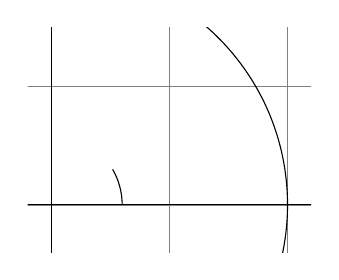
\begin{tikzpicture}[scale=3]
    \clip (-0.1,-0.2) rectangle (1.1,0.75);
    \draw[step=.5cm,gray,very thin] (-1.4,-1.4) grid (1.4,1.4);
    \draw (-1.5,0) -- (1.5,0);
    \draw (0,-1.5) -- (0,1.5);
    \draw (0,0) circle [radius=1cm];
    \draw (3mm,0mm) arc [start angle=0, end angle=30, radius=3mm];
    \end{tikzpicture}
    \end{lstlisting}%
    \end{minipage}
    \begin{minipage}{0.45\textwidth}
    \centering
    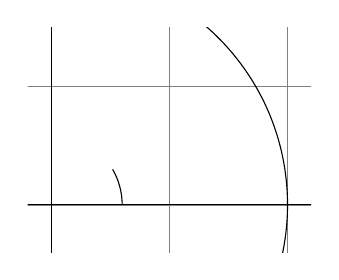
\begin{tikzpicture}[scale=3]
    \clip (-0.1,-0.2) rectangle (1.1,0.75);
    \draw[step=.5cm,gray,very thin] (-1.4,-1.4) grid (1.4,1.4);
    \draw (-1.5,0) -- (1.5,0);
    \draw (0,-1.5) -- (0,1.5);
    \draw (0,0) circle [radius=1cm];
    \draw (3mm,0mm) arc [start angle=0, end angle=30, radius=3mm];
    \end{tikzpicture}
    \end{minipage}
    \end{figure}

    您可同时实现路径绘制与裁剪的双重操作:使用 \backslash draw命令并添加clip选项即可实现(注意:此非完整方案——您也可使用 \backslash clip命令添加draw选项。严格来说,\backslash draw本质是 \backslash path[draw]的简写形式,\backslash clip则是 \backslash path[clip]的简写,因此更底层的实现是 \backslash path[draw,clip])。示例如下:
    \begin{figure}[!hpbt]
    \begin{minipage}{0.5\textwidth}
    \begin{lstlisting}[language=tex]
    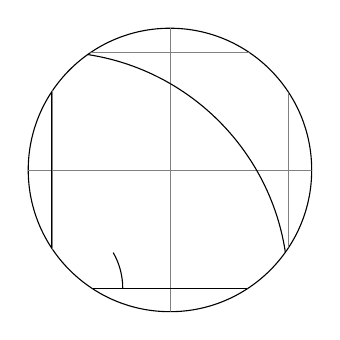
\begin{tikzpicture}[scale=3]
    \clip[draw] (0.5,0.5) circle (.6cm);
    \draw[step=.5cm,gray,very thin] (-1.4,-1.4) grid (1.4,1.4);
    \draw (-1.5,0) -- (1.5,0);
    \draw (0,-1.5) -- (0,1.5);
    \draw (0,0) circle [radius=1cm];
    \draw (3mm,0mm) arc [start angle=0, end angle=30, radius=3mm];
    \end{tikzpicture}
    \end{lstlisting}%
    \end{minipage}
    \begin{minipage}{0.45\textwidth}
    \centering
    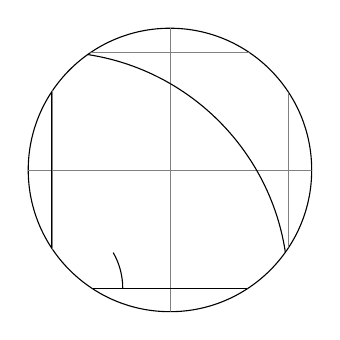
\begin{tikzpicture}[scale=3]
    \clip[draw] (0.5,0.5) circle (.6cm);
    \draw[step=.5cm,gray,very thin] (-1.4,-1.4) grid (1.4,1.4);
    \draw (-1.5,0) -- (1.5,0);
    \draw (0,-1.5) -- (0,1.5);
    \draw (0,0) circle [radius=1cm];
    \draw (3mm,0mm) arc [start angle=0, end angle=30, radius=3mm];
    \end{tikzpicture}
    \end{minipage}
    \end{figure}
    \item \emph{抛物线与正弦路径构建} ~~
    尽管卡尔当前绘图无需这些功能,但他欣喜地发现TikZ提供parabola、sin和cos路径操作符,可在当前路径中追加抛物线及正弦/余弦曲线。抛物线操作的核心特性:当前路径点与操作符后指定的点必在抛物线上。参考以下示例
    \begin{figure}[!hpbt]
    \begin{minipage}{0.5\textwidth}
    \begin{lstlisting}[language=tex]
    \tikz \draw (0,0) rectangle (1,1)  (0,0) parabola (1,1);
    \end{lstlisting}%
    \end{minipage}
    \begin{minipage}{0.45\textwidth}
    \centering
    \tikz \draw (0,0) rectangle (1,1)  (0,0) parabola (1,1);
    \end{minipage}
    \end{figure}

    您还可将弯曲点置于非对称位置:
    \begin{figure}[!hpbt]
    \begin{minipage}{0.5\textwidth}
    \begin{lstlisting}[language=tex]
    \tikz \draw[x=1pt,y=1pt] (0,0) parabola bend (4,16) (6,12);
    \end{lstlisting}%
    \end{minipage}
    \begin{minipage}{0.45\textwidth}
    \centering
    \tikz \draw[x=1pt,y=1pt] (0,0) parabola bend (4,16) (6,12);
    \end{minipage}
    \end{figure}

    sin与cos操作符可在区间内添加正弦/余弦曲线,以前一当前路径点为曲线起点,并以给定终点为曲线终点。示例如下:
    \begin{figure}[!hpbt]
    \begin{minipage}{0.5\textwidth}
    \begin{lstlisting}[language=tex]
    A sine \tikz \draw[x=1ex,y=1ex] (0,0) sin (1.57,1); curve.
    \end{lstlisting}%
    \end{minipage}
    \begin{minipage}{0.45\textwidth}
    \centering
    A sine \tikz \draw[x=1ex,y=1ex] (0,0) sin (1.57,1); curve.
    \end{minipage}
    \end{figure}
    
    \begin{figure}[!hpbt]
    \begin{minipage}{0.5\textwidth}
    \begin{lstlisting}[language=tex]
    \tikz \draw[x=1.57ex,y=1ex] (0,0) sin (1,1) cos (2,0) sin (3,-1) cos (4,0)
                            (0,1) cos (1,0) sin (2,-1) cos (3,0) sin (4,1);
    \end{lstlisting}%
    \end{minipage}
    \begin{minipage}{0.45\textwidth}
    \centering
    \tikz \draw[x=1.57ex,y=1ex] (0,0) sin (1,1) cos (2,0) sin (3,-1) cos (4,0)
                            (0,1) cos (1,0) sin (2,-1) cos (3,0) sin (4,1);
    \end{minipage}
    \end{figure}

    \vskip \baselineskip
    \item \emph{Filling and Drawing} ~~回到图中,卡尔现在希望用极浅的绿色将这个角"填充"起来。为此他没有使用 \backslash draw 命令,而是改用 \backslash fill 命令。卡尔的操作如下:
    \begin{figure}[!hpbt]
    \begin{minipage}{0.5\textwidth}
    \begin{lstlisting}[language=tex]
    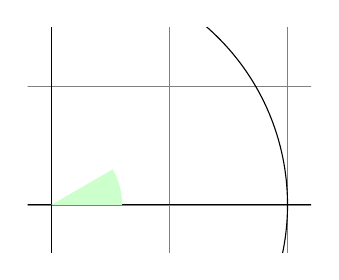
\begin{tikzpicture}[scale=3]
    \clip (-0.1,-0.2) rectangle (1.1,0.75);
    \draw[step=.5cm,gray,very thin] (-1.4,-1.4) grid (1.4,1.4);
    \draw (-1.5,0) -- (1.5,0);
    \draw (0,-1.5) -- (0,1.5);
    \draw (0,0) circle [radius=1cm];
    \fill[green!20!white] (0,0) -- (3mm,0mm)
        arc [start angle=0, end angle=30, radius=3mm] -- (0,0);
    \end{tikzpicture}
    \end{lstlisting}%
    \end{minipage}
    \begin{minipage}{0.45\textwidth}
    \centering
    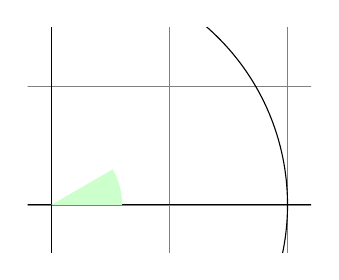
\begin{tikzpicture}[scale=3]
    \clip (-0.1,-0.2) rectangle (1.1,0.75);
    \draw[step=.5cm,gray,very thin] (-1.4,-1.4) grid (1.4,1.4);
    \draw (-1.5,0) -- (1.5,0);
    \draw (0,-1.5) -- (0,1.5);
    \draw (0,0) circle [radius=1cm];
    \fill[green!20!white] (0,0) -- (3mm,0mm)
        arc [start angle=0, end angle=30, radius=3mm] -- (0,0);
    \end{tikzpicture}
    \end{minipage}
    \end{figure}

    颜色表达式 green!20!white 表示 20\% 绿色与 80\% 白色混合(即 20\% 绿色 + 80\% 白色)。之所以能使用此类色彩表达式,是因为 TikZ 底层采用了 Uwe Kern 开发的 xcolor 宏包,具体色彩表达式说明可参阅该宏包的文档。

    如果卡尔最后没有用 \texttt{--(0,0)} 来"闭合"路径会怎样?实际上路径会自动闭合,因此这步操作可以省略。事实上,采用以下写法甚至更为理想
    \begin{verbatim} 
    \fill[green!20!white] (0,0) -- (3mm,0mm)
        arc [start angle=0, end angle=30, radius=3mm] -- cycle;
    \end{verbatim}

    \texttt{--cycle} 指令会将当前路径(实际上是当前路径的当前分段)的首尾点平滑连接形成闭合路径。为直观理解其差异,请看以下示例:
    \begin{figure}[!hpbt]
    \begin{minipage}{0.5\textwidth}
    \begin{lstlisting}[language=tex]
    
\begin{tikzpicture}[line width=5pt]
        \draw (0,0) -- (1,0) -- (1,1) -- (0,0);
        \draw (2,0) -- (3,0) -- (3,1) -- cycle;
        \useasboundingbox (0,1.5); % make bounding box higher
    \end{tikzpicture}
    \end{lstlisting}%
    \end{minipage}
    \begin{minipage}{0.45\textwidth}
    \centering
    
\begin{tikzpicture}[line width=5pt]
        \draw (0,0) -- (1,0) -- (1,1) -- (0,0);
        \draw (2,0) -- (3,0) -- (3,1) -- cycle;
        \useasboundingbox (0,1.5); % make bounding box higher
    \end{tikzpicture}
    \end{minipage}
    \end{figure}

    还可以使用 \backslash filldraw 命令同时执行填充和绘制路径的双重操作。该命令会先绘制路径轮廓,再进行内部填充。初看似乎作用有限,但关键在于可为填充色(fill)和描边色(stroke)分别指定不同颜色。具体通过如下可选参数实现:
    \begin{figure}[!hpbt]
    \begin{minipage}{0.5\textwidth}
    \begin{lstlisting}[language=tex]
    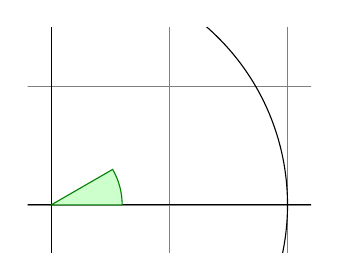
\begin{tikzpicture}[scale=3]
        \clip (-0.1,-0.2) rectangle (1.1,0.75);
        \draw[step=.5cm,gray,very thin] (-1.4,-1.4) grid (1.4,1.4);
        \draw (-1.5,0) -- (1.5,0);
        \draw (0,-1.5) -- (0,1.5);
        \draw (0,0) circle [radius=1cm];
        \filldraw[fill=green!20!white, draw=green!50!black] (0,0) -- (3mm,0mm)
            arc [start angle=0, end angle=30, radius=3mm] -- cycle;
    \end{tikzpicture}
    \end{lstlisting}%
    \end{minipage}
    \begin{minipage}{0.45\textwidth}
    \centering
    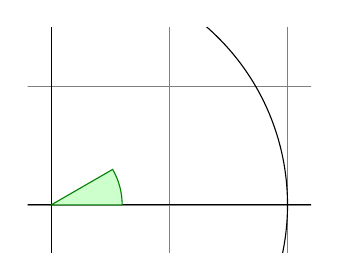
\begin{tikzpicture}[scale=3]
        \clip (-0.1,-0.2) rectangle (1.1,0.75);
        \draw[step=.5cm,gray,very thin] (-1.4,-1.4) grid (1.4,1.4);
        \draw (-1.5,0) -- (1.5,0);
        \draw (0,-1.5) -- (0,1.5);
        \draw (0,0) circle [radius=1cm];
        \filldraw[fill=green!20!white, draw=green!50!black] (0,0) -- (3mm,0mm)
            arc [start angle=0, end angle=30, radius=3mm] -- cycle;
    \end{tikzpicture}
    \end{minipage}
    \end{figure}

    \item \emph{阴影} ~~卡尔短暂考虑过通过着色让这个角显得"更花哨"。与使用单一纯色填充区域不同,着色可实现不同颜色间的平滑渐变。命令如下:
    \begin{figure}[!hpbt]
    \begin{minipage}{0.5\textwidth}
    \begin{lstlisting}[language=tex]
       \tikz \shade (0,0) rectangle (2,1)  (3,0.5) circle (.5cm);
    \end{lstlisting}%
    \end{minipage}
    \begin{minipage}{0.45\textwidth}
    \centering
       \tikz \shade (0,0) rectangle (2,1)  (3,0.5) circle (.5cm);
    \end{minipage}
    \end{figure}
     
    默认着色效果是从灰色到白色的平滑渐变。若需指定其他颜色,可通过以下选项参数实现:
    \begin{figure}[!hpbt]
    \begin{minipage}{0.5\textwidth}
    \begin{lstlisting}[language=tex]
    
\begin{tikzpicture}[rounded corners,ultra thick]
        \shade[top color=yellow,bottom color=black] (0,0) rectangle +(2,1);
        \shade[left color=yellow,right color=black] (3,0) rectangle +(2,1);
        \shadedraw[inner color=yellow,outer color=black,draw=yellow] (6,0) rectangle +(2,1);
        \shade[ball color=green] (9,.5) circle (.5cm);
    \end{tikzpicture}
    \end{lstlisting}%
    \end{minipage}
    \begin{minipage}{0.45\textwidth}
    \centering
    
\begin{tikzpicture}[rounded corners,ultra thick]
        \shade[top color=yellow,bottom color=black] (0,0) rectangle +(2,1);
        \shade[left color=yellow,right color=black] (3,0) rectangle +(2,1);
        \shadedraw[inner color=yellow,outer color=black,draw=yellow] (6,0) rectangle +(2,1);
        \shade[ball color=green] (9,.5) circle (.5cm);
    \end{tikzpicture}
    \end{minipage}
    \end{figure}

    对于卡尔的任务,下面的做法更合适。
    \begin{figure}[!hpbt]
    \begin{minipage}{0.5\textwidth}
    \begin{lstlisting}[language=tex]
    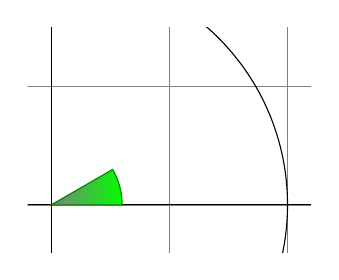
\begin{tikzpicture}[scale=3]
        \clip (-0.1,-0.2) rectangle (1.1,0.75);
        \draw[step=.5cm,gray,very thin] (-1.4,-1.4) grid (1.4,1.4);
        \draw (-1.5,0) -- (1.5,0);
        \draw (0,-1.5) -- (0,1.5);
        \draw (0,0) circle [radius=1cm];
        \shadedraw[left color=gray,right color=green, draw=green!50!black]
            (0,0) -- (3mm,0mm)
            arc [start angle=0, end angle=30, radius=3mm] -- cycle;
    \end{tikzpicture}
    \end{lstlisting}%
    \end{minipage}
    \begin{minipage}{0.45\textwidth}
    \centering
    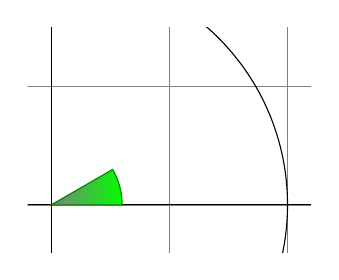
\begin{tikzpicture}[scale=3]
        \clip (-0.1,-0.2) rectangle (1.1,0.75);
        \draw[step=.5cm,gray,very thin] (-1.4,-1.4) grid (1.4,1.4);
        \draw (-1.5,0) -- (1.5,0);
        \draw (0,-1.5) -- (0,1.5);
        \draw (0,0) circle [radius=1cm];
        \shadedraw[left color=gray,right color=green, draw=green!50!black]
            (0,0) -- (3mm,0mm)
            arc [start angle=0, end angle=30, radius=3mm] -- cycle;
    \end{tikzpicture}
    \end{minipage}
    \end{figure}
    然而他明智地决定放弃着色——通常这类效果徒增干扰,对图形表达反而无益。
    \item \emph{指定坐标} ~~卡尔接下来要添加正弦和余弦线。他已知晓可用 color= 选项设置线条颜色,那么如何最优指定坐标位置呢?

    坐标指定存在多种方式。最简易的方法是直接使用 $(10pt,2cm)$ 这类表达式,表示 x轴方向$10pt$、$y$轴方向$2cm$。另一种方式是省略单位写成 $(1,2)$,其含义为"当前$x$向量的$1$倍与当前$y$向量的$2$倍之和"。这两个向量默认值分别为:$x$轴方向$1cm$,$y$轴方向$1cm$。

    要指定极坐标点,可使用 (30:1cm) 格式,表示30度方向上1cm处的点——这在定位"圆周上的点"时尤为实用。

    若在坐标前添加单个"$+$"或双"$++$"符号,如 $+(0cm,1cm)$ 或 $++(2cm,0cm)$,其语义有本质差异:(1)$+$前缀表示“相对前一个坐标点上移$1cm$”;(2) $++$ 前缀表示“相对前一个坐标点右移$2cm$,并将该点更新为新的当前点”。
    \begin{figure}[!hpbt]
    \begin{minipage}{0.5\textwidth}
    \begin{lstlisting}[language=tex]
    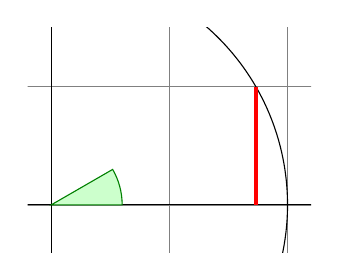
\begin{tikzpicture}[scale=3]
        \clip (-0.1,-0.2) rectangle (1.1,0.75);
        \draw[step=.5cm,gray,very thin] (-1.4,-1.4) grid (1.4,1.4);
        \draw (-1.5,0) -- (1.5,0);
        \draw (0,-1.5) -- (0,1.5);
        \draw (0,0) circle [radius=1cm];
        \filldraw[fill=green!20,draw=green!50!black] (0,0) -- (3mm,0mm)
            arc [start angle=0, end angle=30, radius=3mm] -- cycle;
        \draw[red,very thick] (30:1cm) -- +(0,-0.5);
    \end{tikzpicture}
    \end{lstlisting}%
    \end{minipage}
    \begin{minipage}{0.45\textwidth}
    \centering
    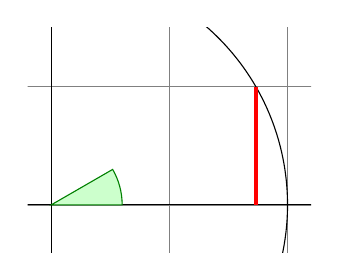
\begin{tikzpicture}[scale=3]
        \clip (-0.1,-0.2) rectangle (1.1,0.75);
        \draw[step=.5cm,gray,very thin] (-1.4,-1.4) grid (1.4,1.4);
        \draw (-1.5,0) -- (1.5,0);
        \draw (0,-1.5) -- (0,1.5);
        \draw (0,0) circle [radius=1cm];
        \filldraw[fill=green!20,draw=green!50!black] (0,0) -- (3mm,0mm)
            arc [start angle=0, end angle=30, radius=3mm] -- cycle;
        \draw[red,very thick] (30:1cm) -- +(0,-0.5);
    \end{tikzpicture}
    \end{minipage}
    \end{figure}

\end{enumerate}





%\section{机器学习绘图}


